%-----------------------------------------------------------------------------%
\chapter{IMPLEMENTASI DAN PENGUJIAN}
%-----------------------------------------------------------------------------%

%
\vspace{4.5pt}
Pada bab ini akan menjelaskan mengenai proses implementasi dan pengujian terhadap sistem yang telah dibangun berdasarkan penjelasan pada bab sebelumnya.\\

\section{Lingkungan Implementasi}
Pada lingkungan implementasi, akan dijelaskan mengenai perangkat yang digunakan dalam proses pembangunan sistem baik dari perangkat keras maupun perangkat lunak yang digunakan.\\

\subsection{Spesifikasi Perangkat Keras}
Spesifikasi komputer yang digunakan dalam pembutan dan pengujian aplikasi deteksi bangunan pada citra udara dengan \textit{Convolutional Neural Network} adalah sebagai berikut:
\begin{enumerate}
	\item Komputer dengan \textit{processor} Intel Core i5-7400U CPU $@$ 2.70GHz
	\item \textit{Harddisk} dengan kapasitas 1 TB
	\item RAM 16 GB
	\item VGA NVDIA GeForce GT 1050M
	\\
\end{enumerate}

\subsection{Lingkungan Perangkat Lunak}
Spesifikasi perangkat lunak yang digunakan dalam pembangunan aplikasi deteksi bangunan pada citra udara dengan \textit{Convolutional Neural Network} adalah sebagai berikut:
7\begin{enumerate}
	\item \textit{Virtual Machine}: VMware Workstation 15
	\item Sistem Operasi: Ubuntu 18.04
	\item IDE: Geany 1.34.1
	\item Development Tool: Python 3.6.8 64-bit
	\\
\end{enumerate}

\section{Daftar Kelas dan Metode}
Pada bagian ini, akan dijelaskan mengenai \textit{class} dan \textit{method} yang digunakan dalam penelitian ini.
\\

\subsection{Daftar \textit{Class} dan \textit{Method} hog\_util\_functions}
Berikut adalah tabel berisi \textit{method} pada \textit{class} hog\_util\_functions. \textit{Class} hog\_util\_functions digunakan untuk mengolah citra menggunakan metode \textit{Histogram of Oriented Gradients}.

\begin{small}
	\begin{longtable}{|p{0.4cm}|p{2.6cm}|p{2cm}|p{2.5cm}|p{1.5cm}|p{4.5cm}|}
		\caption{Daftar Metode pada Kelas \textit{hog\_util\_functions}} \\	
		\hline
		\multirow{2}{*}{\textbf{No}} & \multirow{2}{*}{\textbf{Metode}} & \multicolumn{2}{c|}{\textit{\textbf{Input}}} & \multirow{2}{*}{\textit{\textbf{Output}}} & 
		\multirow{2}{*}{\textbf{Keterangan}}\\
		\cline{3-4}
		& & \textbf{Tipe} & \textbf{Variabel} & & \\
		\hline
		1 & convert\_rgb\_color & string \newline string & img \newline conv & image & Untuk mengubah \textit{color space}.\\
		\hline
		2 & get\_hog\_features & string \newline int \newline int \newline int \newline boolean \newline boolean & img \newline orient \newline pix\_per\_cell \newline cell\_per\_block \newline vis \newline feature\_vec & int[] & Untuk mengambil fitur menggunakan metode HOG.\\
		\hline
		3 & single\_image\_ \newline features & string \newline string \newline int[] \newline int \newline int \newline int \newline int \newline int \newline boolean \newline boolean \newline boolean & img \newline color\_space \newline spatial\_size \newline hist\_bins \newline orient \newline pix\_per\_cell \newline cell\_per\_block \newline hog\_channel \newline spatial\_feat \newline hist\_feat \newline hog\_feat & int[] & Untuk mengekstrak fitur dari satu jendela gambar.\\
		\hline
	\end{longtable}
\end{small}

\subsection{Daftar \textit{Class} dan \textit{Method} find\_cars}
Berikut adalah tabel berisi \textit{method} pada \textit{class} find\_cars. \textit{Class} find\_cars digunakan untuk mencari objek berupa mobil pada frame masukkan.
\begin{small}
	\begin{longtable}{|p{0.4cm}|p{2.6cm}|p{2cm}|p{2.5cm}|p{1.5cm}|p{4.5cm}|}
		\caption{Daftar Metode pada Kelas \textit{find\_cars}} \\	
		\hline
		\multirow{2}{*}{\textbf{No}} & \multirow{2}{*}{\textbf{Metode}} & \multicolumn{2}{c|}{\textit{\textbf{Input}}} & \multirow{2}{*}{\textit{\textbf{Output}}} & 
		\multirow{2}{*}{\textbf{Keterangan}}\\
		\cline{3-4}
		& & \textbf{Tipe} & \textbf{Variabel} & & \\
		\hline
		1 & load\_classifier & string & pickle\_file & int[] & Untuk memuat parameter HOG dan SVM dari \textit{pickle file}.\\
		\hline
		2 & draw\_labeled\_ \newline bboxes & string \newline string \newline int[][][] \newline int & img \newline labels \newline color \newline thick & image & Untuk membuat kotak penanda lokasi mobil yang terdeteksi.\\
		\hline
		3 & find\_cars & string \newline int \newline int \newline int \newline string \newline int \newline string[] \newline int & img \newline ystart \newline ystop \newline scale \newline svc \newline X\_scaler \newline params \newline cells\_per\_step & int[] & Untuk mengekstrak fitur menggunakan sub-sampling HOG dan membuat prediksi.\\
		\hline
	\end{longtable}
\end{small}

\subsection{Daftar \textit{Class} dan \textit{Method} train\_hog\_classifier}
Berikut adalah tabel berisi \textit{method} pada \textit{class} train\_hog\_classifier. \textit{Class} train\_hog\_classifier digunakan untuk proses pelatihan dari dataset.
\begin{small}
	\begin{longtable}{|p{0.4cm}|p{2.6cm}|p{2cm}|p{2.5cm}|p{1.5cm}|p{4.5cm}|}
		\caption{Daftar Metode pada Kelas \textit{train\_hog\_classifier}} \\	
		\hline
		\multirow{2}{*}{\textbf{No}} & \multirow{2}{*}{\textbf{Metode}} & \multicolumn{2}{c|}{\textit{\textbf{Input}}} & \multirow{2}{*}{\textit{\textbf{Output}}} & 
		\multirow{2}{*}{\textbf{Keterangan}}\\
		\cline{3-4}
		& & \textbf{Tipe} & \textbf{Variabel} & & \\
		\hline
		1 & load\_data\_sets &  &  & string[] \newline string[] & Untuk memuat data dari \textit{dataset}.\\
		\hline
		2 & save\_data\_sets & string \newline image[] \newline image[] & pickle\_file \newline cars \newline notcars &  & Untuk menyimpan daftar gambar mobil dan bukan mobil yang sudah dimuat.\\
		\hline
		3 & load\_cars\_norcars & string & data\_file & image[][] \newline image[][] & Untuk memuat \textit{dataset} dari \textit{pickle file}.\\
		\hline
		4 & save\_classifier\_ \newline data & string \newline int \newline int \newline int \newline int & pickle\_file \newline X\_train \newline Y\_train \newline X\_test \newline Y\_test &  & Untuk menyimpan dataset yang sudah dibagi menjadi data latih dan data uji.\\
		\hline
		5 & save\_classifier & string \newline string \newline int \newline string[] & pickle\_file \newline svc \newline X\_scaler \newline params \newline &  & Untuk menyimpan parameter HOG.\\
		\hline
		6 & extract\_features & image \newline string[] & imgs \newline params &  & Untuk mengekstrak fitur dari citra.\\
		\hline
	\end{longtable}
\end{small}

\section{Implementasi Perangkat Lunak}
Pada implementasi perangkat lunak dilakukan menurut analisis yang telah disusun
pada BAB III.\\

\subsection{Implementasi Pengambilan Dataset}
\textit{Dataset} GTI diperoleh dari \textit{http://www.gti.ssr.upm.es/data/Vehicle\_database.html} dan \textit{Dataset} KITTI dari \textit{http://www.cvlibs.net/datasets/kitti/}. Gambar \ref{img:FolderScheme} menunjukkan daftar \textit{folder} penyimpanan \textit{Dataset}.

\begin{table}[H]
	\small
	\begin{adjustbox}{width=1\textwidth}
		\begin{tabular}{| p {14cm} |}
			\hline
			\begin{figure}[H]
				\centering
				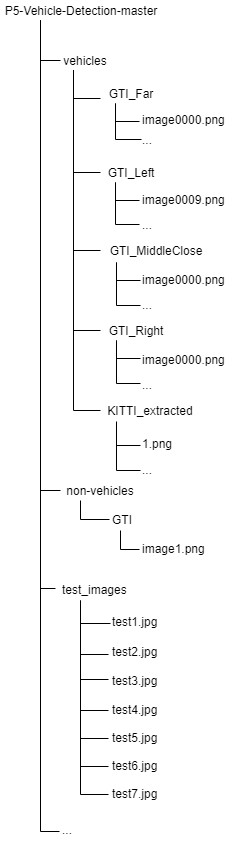
\includegraphics[width=7cm]{images/FolderScheme.png}
			\end{figure} \\
			\hline
		\end{tabular}
	\end{adjustbox}
	\captionof{figure}{Daftar folder \textit{Dataset}}
	\label{img:FolderScheme}
\end{table}  

Citra untuk proses pengenalan kendaraan terbagi menjadi 2 yaitu \textit{vehicles} dan \textit{non-vehicles}. Data citra \textit{vehicles} dibagi menjadi 5 macam yaitu \textit{GTI\_Far, GTI\_Left, GTI\_MiddleClose, GTI\_Right,} dan \textit{KITTI\_extracted}.
\textit{GTI\_Far} berisi citra yang diambil dari jauh. \textit{GTI\_Left} berisi citra yang diambil dari arah kiri kendaraan. \textit{GTI\_MiddleClose} berisi citra yang diambil dari dekat. \textit{GTI\_Right} berisi citra yang diambil dari arah kanan kendaraan. \textit{KITTI\_extracted} berisi citra yang terdiri dari variasi ukuran pengambilan citra. Hasil dari pengumpulan data akan disimpan dalam \textit{pickle file}. Untuk proses klasifikasi, citra dibagi 70\% untuk \textit{training} dan 30\% untuk \textit{testing}. Pembagian citra dilakukan secara acak.

Setelah proses pengenalan kendaraan selesai, hasil pengenalan kemudian digunakan untuk proses deteksi pada \textit{dataset} yang diambil dari \textit{http://www.youtube.com}. Dari \textit{dataset} yang berupa video, sudah terdapat 6 buah citra yang mewakili setiap kondisi pada folder \textit{test\_images}. Gambar \ref{fig:ContohDataDeteksi} menunjukkan citra untuk proses deteksi kendaraan.

\begin{table}[H]
	\small
	\begin{adjustbox}{width=1\textwidth}
		\begin{tabular}{| p {14cm} |}
			\hline
			\begin{figure}[H]
				\centering
				{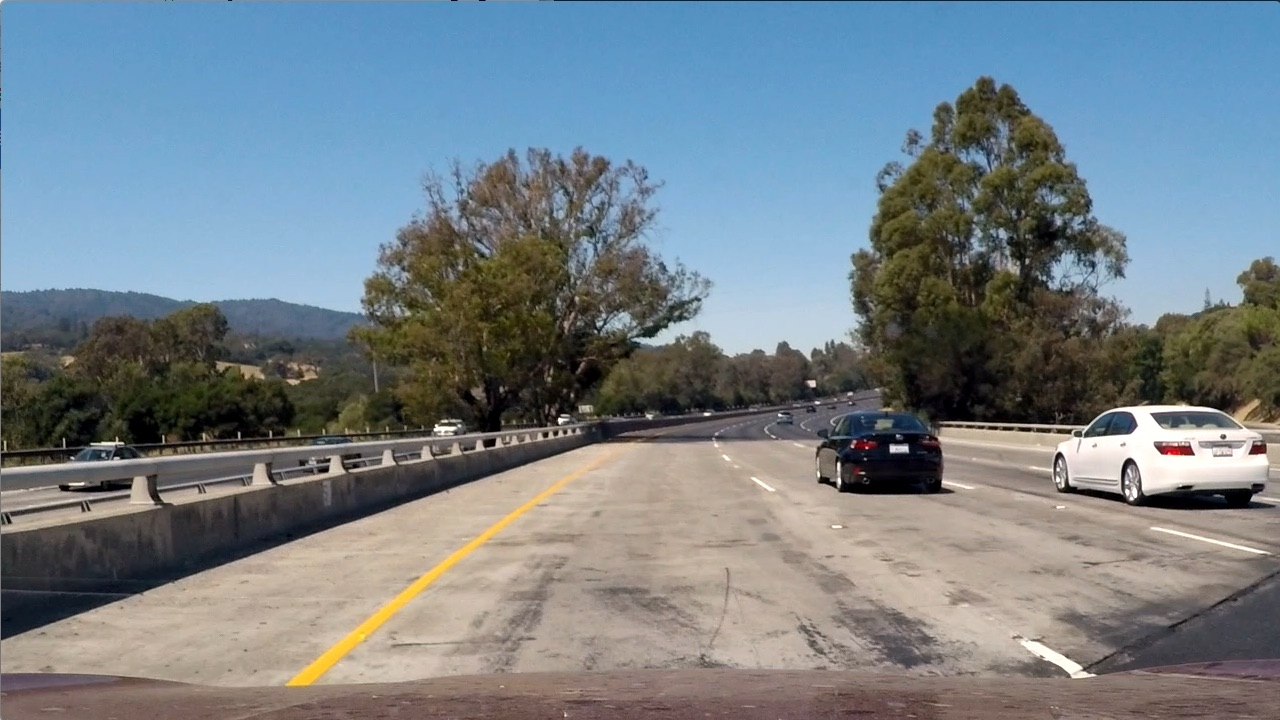
\includegraphics[width = 7cm]{images/test1}} 
				{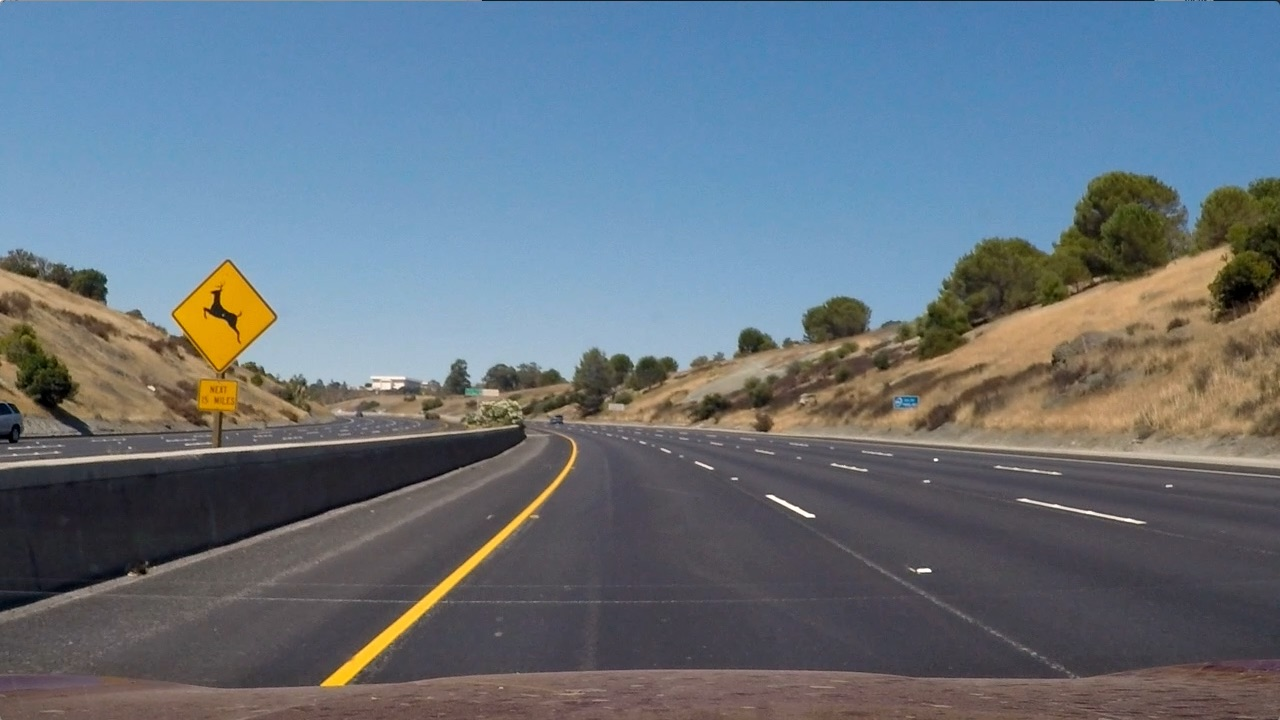
\includegraphics[width = 7cm]{images/test2}} \\
				{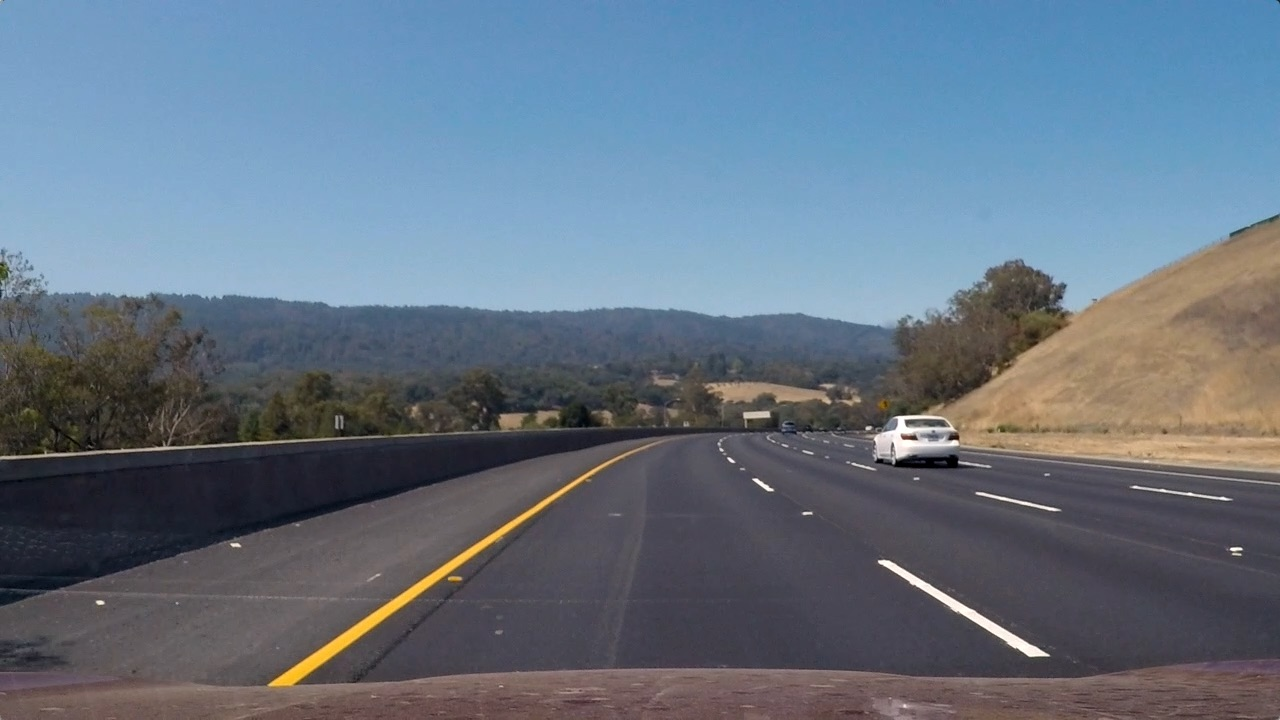
\includegraphics[width = 7cm]{images/test3}}
				{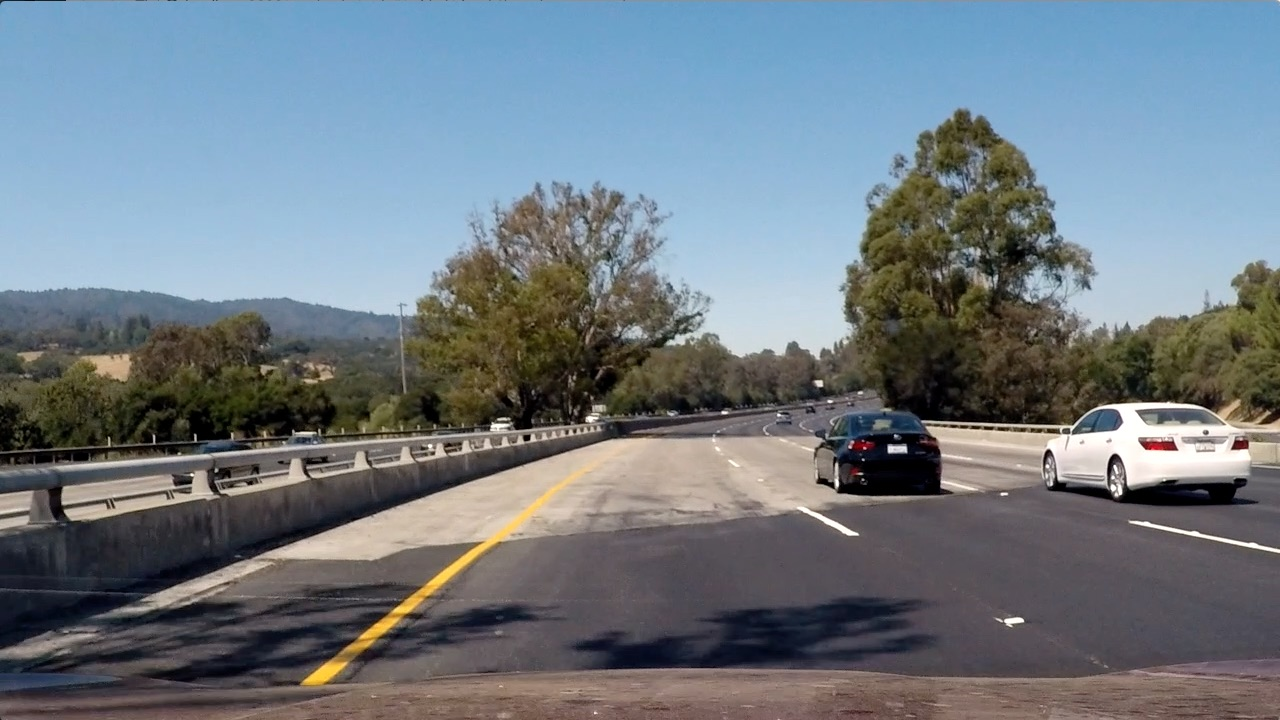
\includegraphics[width = 7cm]{images/test4}}\\
				{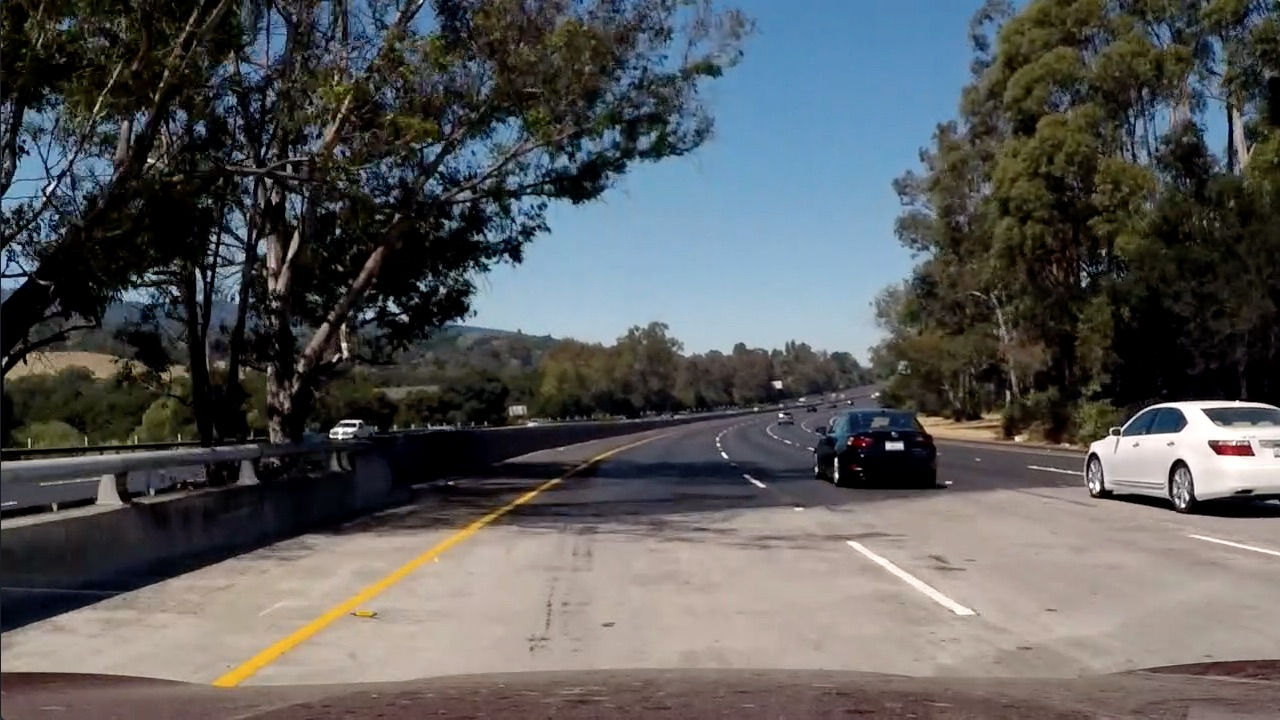
\includegraphics[width = 7cm]{images/test5}}
				{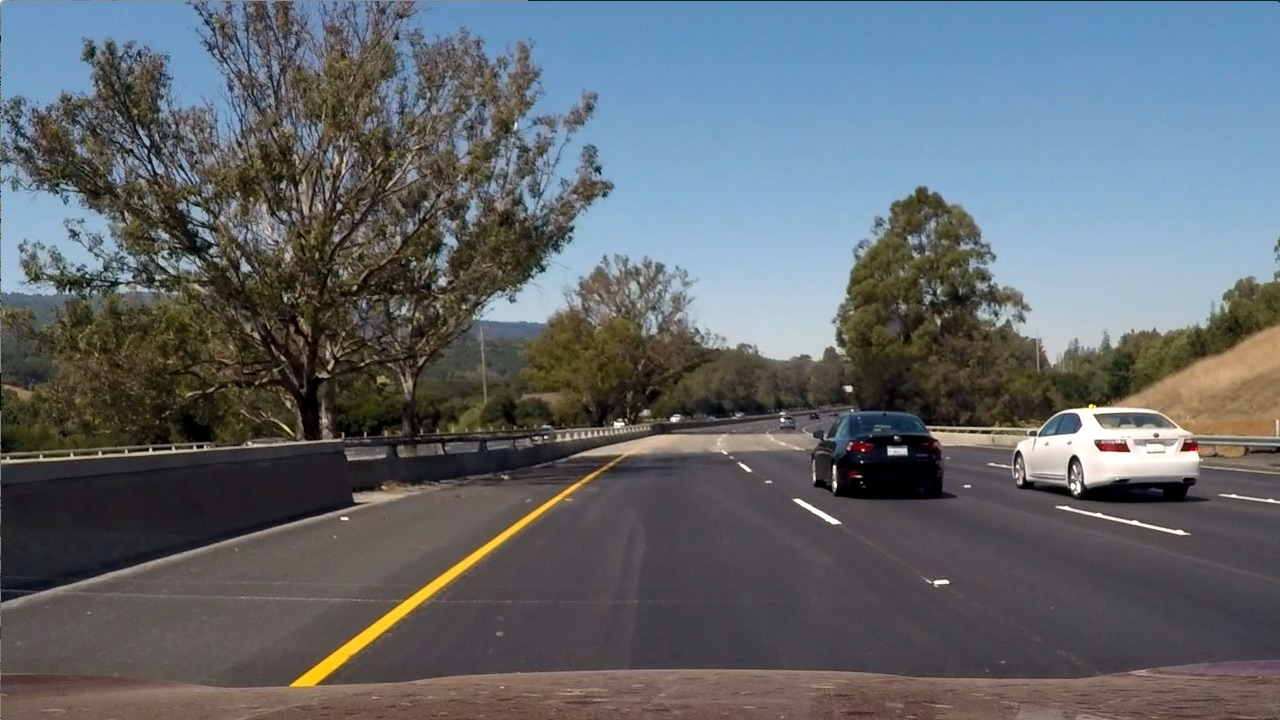
\includegraphics[width = 7cm]{images/test6}}\\
			\end{figure} \\
			\hline
		\end{tabular}
	\end{adjustbox}
	\captionof{figure}{Citra untuk deteksi kendaraan}
	\label{fig:ContohDataDeteksi}
\end{table}

\subsection{Implementasi Proses Latih}
Pelatihan yang dilakukan merupakan proses klasifikasi dimana membedakan objek mobil dan bukan mobil. Berikut ini adalah uraian dari proses pelatihan yang dilakukan dalam penelitian ini:
\begin{enumerate}
	\item \textit{Dataset} dimuat dan dikelompokkan mejadi mobil dan bukan mobil.
	\item Menentukan semua parameter yang dibutuhkan.
	\item Melakukan ekstraksi fitur kepada seluruh \textit{dataset}.
	\item Menyatukan dan melakukan normalisasi terhadap fitur.
	\item Fitur dari \textit{dataset} kemudian diacak dan dibagi menjadi 70\% untuk pelatihan, dan 30\% untuk pengujian.
	\item Melakukan pelatihan proses klasifikasi SVM menggunakan fitur dari data latih.
	\item Menyimpan hasil klasifikasi HOG dalam \textit{pickle file}.
	\\
\end{enumerate}

\subsection{Implementasi Proses Uji}
Pada bagian ini, akan dilakukan berbagai skenario pengujian dengan beragam parameter dari metode HOG. Tujuan dari penelitian ini adalah untuk menerapkan metode \textit{HOG} pada proses ekstraksi fitur, oleh karena itu perlu diketahui beberapa parameter masukkan yaitu ukuran sel, ukuran blok, dan jumlah \textit{bin} untuk menghasilkan fitur dan akurasi pengenalan karakter yang terbaik. Pengujian ini akan dilakukan dengan data latih sebanyak 6 buah citra yang diambil dari video. 6 buah citra ini didapat dari dataset dan sudah meliputi seluruh keadaan kondisi lokasi penelitian.\\

\subsection{Implementasi Aplikasi}
Bagian ini menjelaskan tampilan \textit{Graphical User Interface} (GUI) yang terdapat dalam aplikasi deteksi mobil dari citra kamera yang diambil dari \textit{dashboard} mobil. Tampulan GUI berguna untuk memudahkan user dalam melakukan proses uji. Tampilan dibuat berbasis \textit{desktop} menggunakan bahasa program python. Berikut adalah tampilan dari aplikasi deteksi mobil:
\\

\subsection{Skenario Pengujian}
Pada tahap ini, akan dijelaskan mengenai pengujian yang dilakukan dengan aplikasi yang telah dibuat. Hasil dari pengujian ini adalah untuk mendapatkan hasil klasifikasi untuk deteksi mobil menggunakan metode HOG.
\\

\subsubsection{Pengujian Kombinasi Parameter}
Bagian ini akan menjelaskan pengujian dengan beragam kombinasi parameter metode HOG dalam proses ekstraksi fitur. Fitur dari metode \textit{HOG} akan digunakan pada proses klasifikasi dan deteksi dengan nilai dari setiap parameter yang akan digunakan untuk kombinasi meliputi:
\begin{enumerate}
	\item Ukuran sel yang akan digunakan : 2, 4, 8, 16
	\item Ukuran blok yang akan digunakan : 4, 8, 16, 32
	\item Jumlah \textit{bin} yang akan digunakan : 4, 6, 9, 18
\end{enumerate}
Untuk nilai sigma pada metode \textit{SVM} yang digunakan dalam kombinasi adalah 0.01, 0.1, dan 1. Hasil kemudian akan diukur akurasinya menggunakan \textit{Confusion Matrix}.\\

\subsubsection{Pengujian dengan Ukuran Sel 2}
Bagian ini akan menjelaskan pengujian terhadap akurasi dengan menggunakan ukuran sel 2 $\times$ 2 piksel dan ukuran blok 2 $\times$ 2 sel (4 $\times$ 4 piksel). Dalam penelitian ini, jumlah bin yang akan digunakan adalah 4, 6, 9, dan 18 dan untuk nilai sigma pada metode \textit{SVM} yang akan digunakan adalah 0.01, 0.1, dan 1. Berikut adalah hasil pengujian untuk setiap kombinasi parameter tersebut:
\begin{longtable}[c]{|c|c|c|}
	\caption{Hasil Pengujian dengan ukuran sel 2 $\times$ 2 piksel}
	\label{tab:HasilPengujianSel2}\\
	\hline
	\begin{tabular}[c]{@{}c@{}}Parameter\\ (CellSize, NumBins, Sigma)\end{tabular} & CRR     & OVR     \\ \hline
	\endhead
	%
	(2, 4, 0.01)                                                                   & {\color[HTML]{FE0000} 58.52\%} & {\color[HTML]{FE0000} 10.34\%} \\ \hline
	(2, 4, 0.1)                                                                    & 26.13\% & 0\%     \\ \hline
	(2, 4, 1)                                                                      & 18.18\% & 0\%     \\ \hline
	(2, 6, 0.01)                                                                   & 50\%    & 6.89\%  \\ \hline
	(2, 6, 0.1)                                                                    & 25.56\% & 0\%     \\ \hline
	(2, 6, 1)                                                                      & 18.18\% & 0\%     \\ \hline
	(2, 9, 0.01)                                                                   & 48.29\% & 3.44\%  \\ \hline
	(2, 9, 0.1)                                                                    & 25\%    & 0\%     \\ \hline
	(2, 9, 1)                                                                      & 18.18\% & 0\%     \\ \hline
	(2, 18, 0.01)                                                                  & 44.88\% & 3.44\%  \\ \hline
	(2, 18, 0.1)                                                                   & 25\%    & 0\%     \\ \hline
	(2, 18, 1)                                                                     & 18.18\% & 0\%     \\ \hline
\end{longtable}
Berdasarkan tabel di atas, dapat disimpulkan bahwa akurasi pengenalan karakter maksimal yang didapatkan apabila menggunakan ukuran sel 2 $\times$ 2 piksel adalah 58.52\%. Kombinasi parameter yang digunakan untuk mencapai hasil tersebut adalah ukuran sel 2 $\times$ 2 piksel, jumlah \textit{bin} sebanyak 4 sehingga besar setiap \textit{bin} adalah 45 derajat, kemudian nilai \textit{sigma} yang digunakan untuk metode \textit{SVM} adalah 0.01. Dengan citra karakter inputan berukuran 32 $\times$ 32 piksel. Maka panjang vektor fitur dari \textit{HOG descriptor} yang dihasilkan adalah 3600 fitur.

Kolom di bagian kiri menunjukkan kombinasi parameter yang digunakan pada saat pengujian. Kolom CRR merupakan akronim dari \textit{Character Recognition Rate} yang memiliki rumus jumlah karakter yang dikenali dibagi dengan keseluruhan karakter yang terdeteksi. Dari 176 karakter yang terdeteksi, sebanyak 103 di antaranya dapat diklasifikasikan dengan baik. Kolom OVR pada bagian kanan menunjukkan performa keseluruhan yang memiliki rumus jumlah plat nomor yang terdeteksi dan dikenali dengan benar dibagi dengan keseluruhan jumlah plat nomor yang ada. Dari 29 plat nomor yang terdeteksi, hanya 3 plat nomor yang dapat dikenali dengan baik. Dapat disimpulkan bahwa penggunaan ukuran sel 2 $\times$ 2 piksel kurang tepat untuk kasus ini.\\

\subsubsection{Pengujian dengan Ukuran Sel 4}
Pada bagian ini, pengujian akan dilakukan dengan menggunakan ukuran sel berukuran 4 $\times$ 4 piksel dan ukuran blok 2 $\times$ 2 sel (8 $\times$ 8 piksel). Jumlah bin yang akan digunakan adalah 4, 6, 9, dan 18. Sedangkan untuk nilai sigma pada metode \textit{SVM} yang akan digunakan adalah 0.01, 0.1, dan 1. Berikut adalah hasil pengujian untuk setiap kombinasi parameter tersebut:
\begin{longtable}[c]{|c|c|c|}
	\caption{Hasil Pengujian dengan ukuran sel 4 $\times$ 4 piksel}
	\label{tab:HasilPengujianSel4}\\
	\hline
	\begin{tabular}[c]{@{}c@{}}Parameter\\ (CellSize, NumBins, Sigma)\end{tabular} & CRR     & OVR     \\ \hline
	\endhead
	%
	(4, 4, 0.01)                                                                   & 86.36\% & 27.58\% \\ \hline
	(4, 4, 0.1)                                                                    & 47.72\% & 0\%     \\ \hline
	(4, 4, 1)                                                                      & 26.13\% & 0\%     \\ \hline
	(4, 6, 0.01)                                                                   & 85.22\% & 31.03\%  \\ \hline
	(4, 6, 0.1)                                                                    & 40.90\% & 0\%     \\ \hline
	(4, 6, 1)                                                                      & 25\%    & 0\%     \\ \hline
	(4, 9, 0.01)                                                                   & {\color[HTML]{FE0000} 89.77\%} & {\color[HTML]{FE0000} 37.93\%}  \\ \hline
	(4, 9, 0.1)                                                                    & 40.90\% & 0\%     \\ \hline
	(4, 9, 1)                                                                      & 23.86\% & 0\%     \\ \hline
	(4, 18, 0.01)                                                                  & 84.09\% & 34.48\%  \\ \hline
	(4, 18, 0.1)                                                                   & 40.90\% & 0\%     \\ \hline
	(4, 18, 1)                                                                     & 24.43\% & 0\%     \\ \hline
\end{longtable}
Berdasarkan tabel di atas, dapat disimpulkan bahwa akurasi pengenalan karakter maksimal yang didapatkan apabila menggunakan ukuran sel 4 $\times$ 4 piksel adalah 89.77\%. Kombinasi parameter yang digunakan untuk mencapai hasil tersebut adalah ukuran sel 4 $\times$ 4 piksel, jumlah \textit{bin} sebanyak 9 sehingga besar setiap \textit{bin} adalah 20 derajat, kemudian nilai \textit{sigma} yang digunakan untuk metode \textit{SVM} adalah 0.01. Dengan citra karakter inputan berukuran 32 $\times$ 32 piksel. Maka panjang vektor fitur dari \textit{HOG descriptor} yang dihasilkan adalah 1764 fitur. Jika dibandingkan dengan pengujian sebelumnya, jumlah fitur yang lebih sedikit justru mampu mendapatkan akurasi pengenalan karakter yang lebih baik.

Sama seperti bagian sebelumnya, kolom di bagian kiri menunjukkan kombinasi parameter yang digunakan pada saat pengujian. Dari hasil pada kolom CRR, dari 176 karakter yang terdeteksi, sebanyak 158 di antaranya dapat diklasifikasikan dengan baik. Dari hasil pada kolom OVR menunjukkan, dari 29 plat nomor yang terdeteksi, 11 plat nomor dapat dikenali dengan baik, hal ini merupakan peningkatan apabila dibandingkan dengan hasil pengujian sebelumnya, namun masih cukup banyak plat yang tidak dapat dikenali dengan baik. Dari pengujian ini dapat  disimpulkan bahwa penggunaan ukuran sel 4 $\times$ 4 piksel sudah dapat meningkatkan akurasi pengenalan karakter namun masih belum optimal.\\

\subsubsection{Pengujian dengan Ukuran Sel 8}
Pada bagian ini, pengujian akan dilakukan dengan menggunakan ukuran sel berukuran 8 $\times$ 8 piksel dan ukuran blok 2 $\times$ 2 sel (16 $\times$ 16 piksel). Jumlah bin yang akan digunakan adalah 4, 6, 9, dan 18. Sedangkan untuk nilai sigma pada metode \textit{SVM} yang akan digunakan adalah 0.01, 0.1, dan 1. Berikut adalah hasil pengujian untuk setiap kombinasi parameter tersebut:
\begin{longtable}[c]{|c|c|c|}
	\caption{Hasil Pengujian dengan ukuran sel 8 $\times$ 8 piksel}
	\label{tab:HasilPengujianSel8}\\
	\hline
	\begin{tabular}[c]{@{}c@{}}Parameter\\ (CellSize, NumBins, Sigma)\end{tabular} & CRR     & OVR     \\ \hline
	\endhead
	%
	(8, 4, 0.01)                                                                   & 15.90\% & 0\% \\ \hline
	(8, 4, 0.1)                                                                    & 93.18\% & 51.72\%     \\ \hline
	(8, 4, 1)                                                                      & 46.02\% & 0\%     \\ \hline
	(8, 6, 0.01)                                                                   & 21.02\% & 0\%  \\ \hline
	(8, 6, 0.1)                                                                    & 93.18\% & 51.72\%     \\ \hline
	(8, 6, 1)                                                                      & 42.61\% & 0\%     \\ \hline
	(8, 9, 0.01)                                                                   & 28.40\% & 0\%  \\ \hline
	(8, 9, 0.1)                                                                    & 93.75\% & 51.72\%     \\ \hline
	(8, 9, 1)                                                                      & 39.20\% & 0\%     \\ \hline
	(8, 18, 0.01)                                                                  & 21.59\% & 0\%  \\ \hline
	(8, 18, 0.1)                                                                   & {\color[HTML]{FE0000} 94.88\%} & {\color[HTML]{FE0000} 58.62\%}     \\ \hline
	(8, 18, 1)                                                                     & 40.34\% & 0\%     \\ \hline
\end{longtable}
Berdasarkan tabel di atas, dapat disimpulkan bahwa akurasi pengenalan karakter maksimal yang didapatkan apabila menggunakan ukuran sel 8 $\times$ 8 piksel adalah 94.88\%. Kombinasi parameter yang digunakan untuk mencapai hasil tersebut adalah ukuran sel 8 $\times$ 8 piksel, jumlah \textit{bin} sebanyak 18 sehingga besar setiap \textit{bin} adalah 10 derajat, kemudian nilai \textit{sigma} yang digunakan untuk metode \textit{SVM} adalah 0.1. Dengan citra karakter inputan berukuran 32 $\times$ 32 piksel. Maka panjang vektor fitur dari \textit{HOG descriptor} yang dihasilkan adalah 648 fitur. Sama seperti pengujian sebelumnya, jika dibandingkan dengan pengujian sebelumnya, jumlah fitur yang lebih sedikit justru mampu mendapatkan akurasi pengenalan karakter yang lebih baik.

Sama seperti bagian sebelumnya, kolom di bagian kiri menunjukkan kombinasi parameter yang digunakan pada saat pengujian. Dari hasil pada kolom CRR, dari 176 karakter yang terdeteksi, sebanyak 167 di antaranya dapat diklasifikasikan dengan baik. Dari hasil pada kolom OVR menunjukkan, dari 29 plat nomor yang terdeteksi, 17 plat nomor dapat dikenali dengan baik, hal ini merupakan peningkatan apabila dibandingkan dengan hasil pengujian sebelumnya, dengan memperhatikan akurasi pengenalan karakter yang tinggi namun hasil performa keseluruhan yang masih di bawah 70\% maka dapat disimpulkan bahwa kemungkinan ada faktor lain yang cukup menghambat dalam proses pengenalan karakter pada keseluruhan plat nomor. Dari pengujian ini dapat  disimpulkan bahwa penggunaan ukuran sel 8 $\times$ 8 piksel sudah dapat menghasilkan akurasi pengenalan karakter yang baik.\\

\subsubsection{Pengujian dengan Ukuran Sel 16}
Pada bagian ini, pengujian akan dilakukan dengan menggunakan ukuran sel berukuran 16 $\times$ 16 piksel dan ukuran blok 2 $\times$ 2 sel (32 $\times$ 32 piksel). Jumlah bin yang akan digunakan adalah 4, 6, 9, dan 18. Sedangkan untuk nilai sigma pada metode \textit{SVM} yang akan digunakan adalah 0.01, 0.1, dan 1. Berikut adalah hasil pengujian untuk setiap kombinasi parameter tersebut:
\begin{longtable}[c]{|c|c|c|}
	\caption{Hasil Pengujian dengan ukuran sel 16 $\times$ 16 piksel}
	\label{tab:HasilPengujianSel16}\\
	\hline
	\begin{tabular}[c]{@{}c@{}}Parameter\\ (CellSize, NumBins, Sigma)\end{tabular} & CRR     & OVR     \\ \hline
	\endhead
	%
	(16, 4, 0.01)                                                                   & 13.06\% & 0\% \\ \hline
	(16, 4, 0.1)                                                                    & 18.75\% & 0\%     \\ \hline
	(16, 4, 1)                                                                      & 84.09\% & 17.24\%     \\ \hline
	(16, 6, 0.01)                                                                   & 13.06\% & 0\%  \\ \hline
	(16, 6, 0.1)                                                                    & 22.72\% & 0\%     \\ \hline
	(16, 6, 1)                                                                      & 84.09\% & 13.79\%     \\ \hline
	(16, 9, 0.01)                                                                   & 13.06\% & 0\%  \\ \hline
	(16, 9, 0.1)                                                                    & 28.97\% & 0\%     \\ \hline
	(16, 9, 1)                                                                      & {\color[HTML]{FE0000} 86.36\%} & {\color[HTML]{FE0000} 27.58\%}     \\ \hline
	(16, 18, 0.01)                                                                  & 13.06\% & 0\%  \\ \hline
	(16, 18, 0.1)                                                                   & 23.29\% & 0\%     \\ \hline
	(16, 18, 1)                                                                     & 85.79\% & 24.13\%     \\ \hline
\end{longtable}
Berdasarkan tabel di atas, dapat disimpulkan bahwa akurasi pengenalan karakter maksimal yang didapatkan apabila menggunakan ukuran sel 16 $\times$ 16 piksel adalah 86.36\%. Kombinasi parameter yang digunakan untuk mencapai hasil tersebut adalah ukuran sel 16 $\times$ 16 piksel, jumlah \textit{bin} sebanyak 9 sehingga besar setiap \textit{bin} adalah 20 derajat, kemudian nilai \textit{sigma} yang digunakan untuk metode \textit{SVM} adalah 1. Dengan citra karakter inputan berukuran 32 $\times$ 32 piksel. Maka panjang vektor fitur dari \textit{HOG descriptor} yang dihasilkan adalah 9 fitur. Berbeda dengan pengujian sebelumnya, kali ini jumlah fitur yang terlalu sedikit justru akan mengurangi akurasi dari proses pengenalan karakter yang sebelumnya sudah mencapai 94.88\%, dari keseluruhan pengujian yang sudah dilakukan terhadap jumlah sel, dapat disimpulkan bahwa ukuran sel yang terlampau besar ataupun terlampau kecil pada penggunaan metode \textit{HOG} dapat mengurangi kualitas fitur yang dihasilkan sehingga akan berefek terhadap hasil klasifikasi.

Sama seperti bagian sebelumnya, kolom di bagian kiri menunjukkan kombinasi parameter yang digunakan pada saat pengujian. Dari hasil pada kolom CRR, dari 176 karakter yang terdeteksi, sebanyak 152 di antaranya dapat diklasifikasikan dengan baik. Dari hasil pada kolom OVR menunjukkan, dari 29 plat nomor yang terdeteksi, 8 plat nomor dapat dikenali dengan baik, hal ini merupakan dampak dari penurunan akurasi pengenalan karakter. Dari pengujian ini dapat  disimpulkan bahwa penggunaan ukuran sel 16 $\times$ 16 piksel dapat menghasilkan akurasi pengenalan karakter yang baik namun belum optimal.\\

\newpage